\documentclass{article}

% EE265B Final Project Report — CoRL 2026 style, preprint mode (no conference footnote)
\usepackage[preprint]{corl_2026}

\usepackage{graphicx}
\usepackage{booktabs}
\usepackage{amsmath,amssymb}
\usepackage{xcolor}
\usepackage{tikz}
\usetikzlibrary{positioning,arrows.meta,fit,calc}

% ---------- placeholder helpers ----------
% red TBD marker for numbers/info the author will fill in
\newcommand{\tbd}[1]{\textcolor{red}{[TBD: #1]}}
% framed figure placeholder: \figslot{<height>}{<what to capture>}
\newcommand{\figslot}[2]{%
  \fbox{\begin{minipage}[c][#1][c]{0.94\linewidth}\centering
    \textcolor{red}{\textbf{[FIGURE SLOT]}}\\[2pt]
    \textcolor{red}{\small #2}
  \end{minipage}}}

\title{Correcting Symbolic Subgoals with Perceptual Memory:\\
A Dual-Memory Policy for Long-Horizon Counting Manipulation}

\author{
  Hefeifei Jiang\\
  EE265B Final Project\\
  University of California, Riverside\\
  \texttt{\tbd{email}}
}

\begin{document}
\maketitle

%===============================================================================

\begin{abstract}
Long-horizon manipulation tasks are often non-Markovian: the current observation alone cannot tell a robot how far it has progressed. Counting tasks expose this dependence in its purest form---a policy must repeat a sub-task exactly $N$ times and then stop, while every repetition leaves the scene looking nearly identical. The recent RoboMME benchmark shows that no single memory representation solves such tasks: symbolic subgoals carry the count explicitly but rely on an error-prone vision--language model (VLM), while perceptual memory is robust but never represents the count directly. We propose a \emph{dual-memory} vision--language--action (VLA) policy that combines both pathways and, crucially, uses perceptual memory to \emph{correct} the symbolic pathway: a learned token-wise gate suppresses subgoal information when it conflicts with visual evidence, and a stale-subgoal augmentation teaches the policy to recognize outdated subgoals during training. On the PickXTimes counting task, our experiments surface three findings that we argue matter more than the raw success rates: (i) VLM-generated subgoals fail in a structured way, drifting and repeating stale stages; (ii) perceptual memory is most valuable as a \emph{verification} signal layered on top of symbolic memory rather than as a replacement for it; and (iii) VLM-based verification is effective but computationally expensive, motivating lightweight learned verifiers as a path forward.
\end{abstract}

\keywords{Memory, Vision-Language-Action Models, Long-Horizon Manipulation}

%===============================================================================
\section{Introduction}
\label{sec:intro}

Most robot manipulation research targets short-horizon skills: grasp a cup, insert a plug, open a drawer. A single observation usually contains everything the policy needs, and once the skill succeeds the episode ends. Long-horizon tasks break this assumption. When a robot must tidy a table or repeat a pick-and-place motion $N$ times, task progress stretches across hundreds of control steps, and the task becomes \emph{non-Markovian}: the current camera frame no longer reveals \emph{where in the task} the robot is. The policy must remember---how many repetitions are done, what it saw earlier, which sub-task comes next.

Counting tasks isolate this difficulty in its cleanest form. In the PickXTimes task of the RoboMME benchmark~\cite{robomme2026}, a robot must pick and place a cube a specified number of times and then press a button to stop. After every repetition the scene returns to a visually near-identical configuration; the only quantity separating ``done twice'' from ``done three times'' is an internal count $k$ that exists nowhere in the pixels. Success is binary and interpretable---either the policy kept count or it lost it---which makes counting an ideal probe for studying memory mechanisms in isolation.

RoboMME equips a shared $\pi_{0.5}$ backbone~\cite{pi05} with three families of memory representation and evaluates each \emph{in isolation}: \emph{symbolic} memory stores history as language subgoals written by an auxiliary VLM; \emph{perceptual} memory stores compressed visual tokens from past frames; \emph{recurrent} memory compresses history into a fixed-size latent state. Its central finding is that no single representation dominates---each carries the count $k$ in a different and differently flawed way. Symbolic memory can state the count explicitly (``placed 2 of 3'') but inherits the instability of the VLM that writes it: in realistic settings the VLM miscounts, and reported counting performance drops far below what the same representation achieves with oracle subgoals. Perceptual memory is learned end-to-end and needs no external model, but the count is never written anywhere---it must \emph{emerge} from a stack of near-identical frames.

These two failure modes are complementary, which suggests an obvious question that RoboMME leaves open: \textbf{what happens when the two representations are combined---and can one repair the other?} This report describes a dual-memory VLA policy built to answer that question on PickXTimes. Symbolic grounded subgoals enter through the language prompt; perceptual frame-sampling memory modulates the action expert; and a learned token-wise \emph{correction gate} lets visual evidence suppress the symbolic pathway when the subgoal is wrong or outdated. Because the dominant VLM failure we observed is \emph{staleness}---the VLM re-emitting a subgoal from several steps ago---we additionally introduce a \emph{stale-subgoal augmentation} that injects outdated subgoals during training, teaching the policy what an untrustworthy subgoal looks like.

We make three contributions:
\begin{enumerate}
  \item \textbf{A dual-memory architecture on RoboMME.} To our knowledge this is the first attempt to combine symbolic and perceptual memory representations within the RoboMME/MME-VLA framework, where all fourteen released variants use a single representation. The design reuses each representation's strongest integration mechanism (subgoals as prompt context; perceptual tokens as action-expert modulation), merges two independently trained checkpoints with a dedicated weight loader, and fine-tunes only lightweight adapter modules.
  \item \textbf{A correction mechanism for unreliable subgoals.} A token-wise sigmoid gate, initialized to suppress memory, learns when perceptual evidence should override symbolic content, complemented by a stale-subgoal training augmentation that simulates the VLM's real failure distribution.
  \item \textbf{An empirical analysis of \emph{why} the symbolic pathway fails.} Through case studies on PickXTimes rollouts we characterize VLM subgoal drift and stale repetition, show that perceptual information is most useful as a verification layer, and quantify the practical cost of VLM-based verification---findings we believe are more transferable than any single success-rate number.
\end{enumerate}

%===============================================================================
\section{Related Work}
\label{sec:related}

\textbf{Vision--language--action models.} Large VLA policies map raw observations and language instructions directly to robot actions. Representative systems include OpenVLA~\cite{openvla} and the $\pi_0$/$\pi_{0.5}$ family~\cite{pi0,pi05}, which couple a pretrained vision--language backbone with a flow-matching action expert; low-level imitation learners such as ACT~\cite{act} and Diffusion Policy~\cite{diffusionpolicy} established the action-chunking foundations these systems build on. These models are predominantly \emph{Markovian}: they condition on the current observation (or a short window) and struggle on history-dependent tasks, which is precisely the regime this report targets.

\textbf{Memory for manipulation policies.} A growing line of work augments VLAs with memory. MemoryVLA~\cite{memoryvla} maintains a perceptual--cognitive memory bank for long-horizon manipulation; MemER~\cite{memer} retrieves keyframes from episodic experience and is the strongest external method on RoboMME; RMBench~\cite{rmbench} classifies tasks by how many past observations must be retained. Recurrent mechanisms such as Recurrent Memory Transformers~\cite{rmt} and test-time-training layers~\cite{ttt} compress history into fixed-size states but were found unstable when grafted onto a pretrained VLA~\cite{robomme2026}. RoboMME~\cite{robomme2026} provides the systematic study our work builds on: a taxonomy of temporal, spatial, object, and procedural memory, sixteen ManiSkill tasks~\cite{maniskill3}, and fourteen memory-augmented variants of $\pi_{0.5}$ crossing three representations with three integration mechanisms under a fixed 512-token budget. All fourteen variants employ a \emph{single} representation; the authors explicitly note the representations are complementary and call for unified designs, which is the gap we address.

\textbf{Language subgoals and their correction.} Using language as an intermediate plan has a long history, from SayCan~\cite{saycan} and Inner Monologue~\cite{innermonologue} to RoboMME's symbolic memory, where a VLM (Gemini~\cite{gemini25} or a fine-tuned Qwen-VL~\cite{qwen25vl}) writes grounded subgoals such as ``pick up the green cube at $[63,152]$.'' The reliability of such generated language is a known weakness: DROC~\cite{droc} distills and retrieves human language corrections, and YAY Robot~\cite{yay} improves long-horizon performance from on-the-fly verbal feedback. Our work differs in that the correction signal is not human language but the policy's \emph{own perceptual memory}, applied in latent space through a learned gate---no human in the loop, and no extra VLM call at correction time.

%===============================================================================
\section{Method}
\label{sec:method}

\subsection{Problem setting: carrying the count}
\label{sec:method-setting}

PickXTimes requires the policy to track a single hidden variable: the number of completed repetitions $k$, to be compared against the instructed target $N$ so the robot continues while $k<N$ and presses the stop button once $k=N$. The two memory pathways we combine carry $k$ in opposite ways:

\begin{itemize}
  \item \textbf{Symbolic (explicit).} An auxiliary VLM observes the rollout and writes a grounded subgoal that encodes the current stage---effectively stating $k$ in language. The form is ideal for counting, but the value is only as reliable as the VLM that writes it.
  \item \textbf{Perceptual (implicit).} A frame-sampling memory retains pooled visual tokens from past observations; the count must be inferred from this visual history. The evidence is grounded and end-to-end trainable, but after each repetition the sampled frames are nearly identical, so the inferred count is fuzzy.
\end{itemize}

Our hypothesis is that these two estimates of the same quantity fail \emph{differently}, so a policy with access to both---plus a mechanism for arbitrating between them---should outperform either alone.

\subsection{Dual-memory architecture}
\label{sec:method-arch}

\begin{figure}[t]
  \centering
  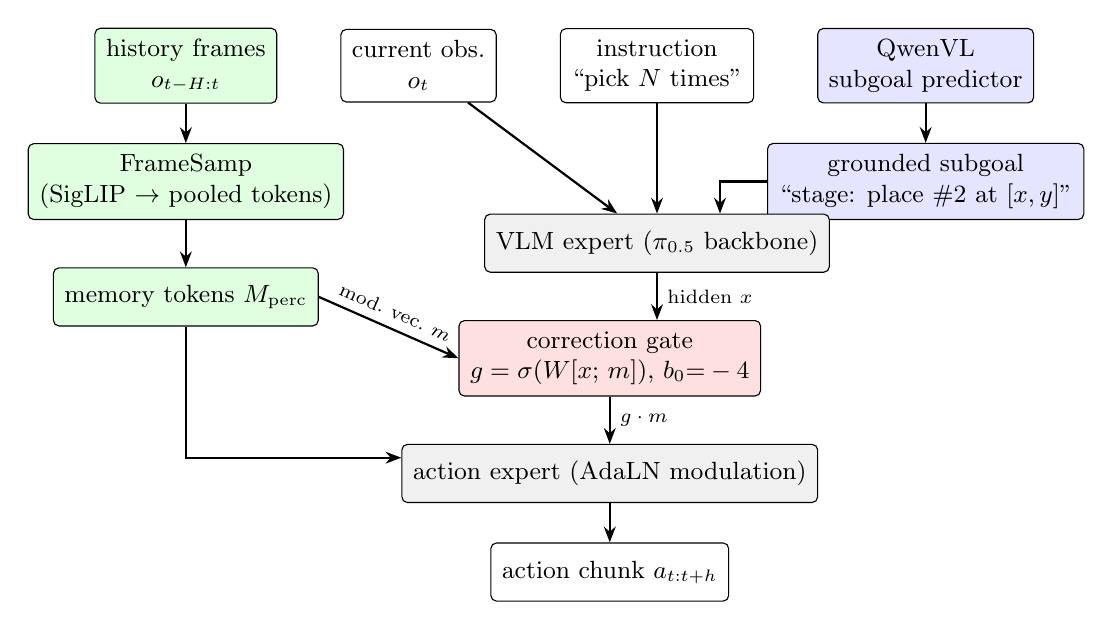
\begin{tikzpicture}[
      font=\small,
      box/.style={draw, rounded corners=2pt, align=center, minimum height=2.1em, inner sep=4pt},
      mem/.style={box, fill=green!12},
      sym/.style={box, fill=blue!10},
      core/.style={box, fill=gray!12},
      gate/.style={box, fill=red!12},
      arr/.style={-{Stealth[length=2mm]}, thick}
    ]
    % inputs
    \node[box] (obs) {current obs.\\$o_t$};
    \node[box, right=8mm of obs] (instr) {instruction\\``pick $N$ times''};
    \node[sym, right=8mm of instr] (vlm) {QwenVL\\subgoal predictor};
    \node[sym, below=5mm of vlm] (subgoal) {grounded subgoal\\``stage: place \#2 at $[x,y]$''};
    % history / perceptual
    \node[mem, left=8mm of obs] (hist) {history frames\\$o_{t-H{:}t}$};
    \node[mem, below=5mm of hist] (framesamp) {FrameSamp\\(SigLIP $\to$ pooled tokens)};
    % vlm expert
    \node[core, below=14mm of instr, minimum width=11em] (vlmexp) {VLM expert ($\pi_{0.5}$ backbone)};
    % modulation + gate
    \node[mem, below=6mm of framesamp] (memtok) {memory tokens $M_{\mathrm{perc}}$};
    \node[gate, below=6mm of vlmexp, xshift=-6mm] (gatebox) {correction gate\\$g=\sigma(W[x;\,m])$, $b_0{=}-4$};
    \node[core, below=6mm of gatebox, minimum width=11em] (actexp) {action expert (AdaLN modulation)};
    \node[box, below=5mm of actexp] (action) {action chunk $a_{t:t+h}$};
    % edges
    \draw[arr] (obs) -- (vlmexp);
    \draw[arr] (instr) -- (vlmexp);
    \draw[arr] (vlm) -- (subgoal);
    \draw[arr] (subgoal) -| ($(vlmexp.north)+(8mm,0)$);
    \draw[arr] (hist) -- (framesamp);
    \draw[arr] (framesamp) -- (memtok);
    \draw[arr] (memtok) |- ($(actexp.west)+(0,2mm)$);
    \draw[arr] (memtok.east) -- node[above, sloped, font=\scriptsize]{mod.\ vec.\ $m$} (gatebox.west);
    \draw[arr] (vlmexp) -- node[right, font=\scriptsize]{hidden $x$} (gatebox.north -| vlmexp.south);
    \draw[arr] (gatebox) -- node[right, font=\scriptsize]{$g\cdot m$} (actexp.north -| gatebox.south);
    \draw[arr] (actexp) -- (action);
  \end{tikzpicture}
  \caption{\textbf{Dual-memory policy with perceptual correction.} The symbolic pathway (blue) injects a VLM-written grounded subgoal into the prompt read by the VLM expert. The perceptual pathway (green) compresses sampled history frames into memory tokens that modulate the action expert through adaptive layer normalization~\cite{adaln}. The token-wise correction gate (red) computes $g\in[0,1]$ from the hidden state and the memory modulation vector and rescales the memory's influence; its bias is initialized to $-4$ so memory is suppressed at the start of fine-tuning.}
  \label{fig:arch}
\end{figure}

Figure~\ref{fig:arch} shows the architecture, implemented on the $\pi_{0.5}$ backbone within the MME-VLA codebase. We deliberately give each representation its strongest integration mechanism as identified by RoboMME:

\textbf{Symbolic pathway (prompt context).} At each control step a Qwen-VL-based subgoal predictor produces a grounded subgoal---a short language string with image coordinates that encodes the current stage of the task. Because subgoals are ordinary language tokens, they are concatenated with the task instruction and consumed by the VLM expert without architectural change. This is the natural integration for symbolic memory and costs only a handful of tokens.

\textbf{Perceptual pathway (action-expert modulation).} A frame-sampling module uniformly subsamples the observation history, encodes each frame with SigLIP~\cite{siglip}, and max-pools the resulting patch grid to a small number of tokens per view under the benchmark's 512-token memory budget. The resulting memory tokens condition the \emph{action expert} through cross-attention followed by adaptive layer normalization (Memory-as-Modulator), the integration RoboMME found strongest for perceptual memory: memory modulates how actions are produced without disturbing the pretrained vision--language stream.

\textbf{Token-wise correction gate.} The gate is the mechanism that lets one memory correct the other. For every token, given the hidden representation $x$ and the perceptual memory modulation vector $m$, the gate computes
\begin{equation}
  g \;=\; \sigma\!\big(W\,[\,x;\,m\,] + b\big) \in [0,1],
  \qquad
  \tilde{m} \;=\; g \cdot m,
\label{eq:gate}
\end{equation}
and the rescaled vector $\tilde{m}$ replaces $m$ in the modulation. The bias is initialized to $b_0=-4$, so $\sigma(b_0)\approx 0.018$: at the start of fine-tuning the perceptual correction is almost silent, and the policy behaves like its symbolic parent. During training the gate learns \emph{when} perceptual evidence disagrees with the symbolic stage---for example, when the subgoal says ``place the second cube'' but the visual history shows the second placement already happened---and opens precisely on those tokens. This realizes correction in latent space with a single linear layer per block, with no extra VLM call.

\subsection{Training recipe}
\label{sec:method-training}

\textbf{Checkpoint merging.} Training a dual policy from scratch would be wasteful: the benchmark already provides strong single-representation checkpoints. A dedicated \texttt{DualMemoryWeightLoader} merges two independently fine-tuned checkpoints (both at step 79{,}999)---one symbolic (GroundSG), one perceptual (FrameSamp+Modul)---by loading the symbolic parameters as the base and overriding all memory-specific modules (\texttt{mem\_encoder}, \texttt{mem\_attn}, \texttt{mem\_rms\_norm}) from the perceptual checkpoint.

\textbf{Adapter-only fine-tuning.} With the merged initialization, we freeze the backbone and train only the lightweight components that arbitrate between pathways: the memory cross-attention adapters, their normalization layers, and the correction gate. Two configurations are used: \emph{dual-lite} (2{,}000 steps; trains the memory adapters so the merged model learns to use both pathways together) and \emph{dual-correction} (500 steps; trains the correction gate on top). Training runs on a single GPU with batch size~1, which makes the entire recipe reproducible on commodity hardware.

\textbf{Stale-subgoal augmentation.} The failure mode that motivates correction must appear in training data, but ground-truth subgoals from demonstrations are always correct. We therefore corrupt them deliberately: with a configured probability, the current subgoal is replaced by a \emph{different subgoal from earlier in the same episode} (bounded lookback, duplicates filtered), simulating the drift-and-repeat behavior we observed in the real QwenVL predictor; grounded coordinates are additionally jittered with Gaussian noise to simulate imperfect grounding. Under this augmentation, the perceptual pathway is the only reliable signal for detecting that the symbolic stage is stale---exactly the skill the gate must learn.

\subsection{Inference-time controllers: VLM-based verification}
\label{sec:method-controllers}

Orthogonal to the learned gate, we also implemented two inference-time subgoal controllers that use \emph{explicit} VLM verification, both to serve as strong baselines and to measure what correction is worth when cost is no object:

\begin{itemize}
  \item \textbf{Progress-verification controller.} After the QwenVL predictor proposes a subgoal, a second VLM call (\texttt{call\_revision}) receives four uniformly sampled recent frames, the candidate subgoal, and the expected stage sequence, and returns a verified or revised subgoal. This catches stage regressions at the price of doubling VLM traffic.
  \item \textbf{Stuck-fallback controller.} A cheaper variant that issues a single VLM call per step and only triggers revision when the output is unparseable, regresses to an earlier stage, or a stage exceeds its time budget (minimum 64/96 steps and timeout 240/280 steps for pick/place respectively). If verification also fails, an internal stage machine generates the subgoal without any VLM.
\end{itemize}

These controllers fix symbolic errors \emph{symbolically}---by asking a VLM to double-check itself against recent frames. The correction gate of Section~\ref{sec:method-arch} can be seen as a learned, amortized replacement for exactly this verification step.

%===============================================================================
\section{Experiments}
\label{sec:experiments}

\subsection{Setup}
\label{sec:exp-setup}

\textbf{Benchmark and task.} All experiments run on RoboMME~\cite{robomme2026}, built on the ManiSkill simulator~\cite{maniskill3} with a 7-DoF Franka Panda, front and wrist RGB cameras, and the benchmark's standard 512-token memory budget. We focus on \textbf{PickXTimes} from the Counting suite: pick and place a colored cube $N$ times, then press the stop button. Episodes run up to 1{,}300 steps; evaluation uses 20 episodes per configuration with held-out seeds (seed 7), and all policies are evaluated at training step 79{,}999 (dual variants fine-tuned from merged checkpoints as in Section~\ref{sec:method-training}).

\begin{figure}[t]
  \centering
  \figslot{11em}{Screenshot slot — \textbf{PickXTimes rollout storyboard}: 6--8 frames from one successful episode (front camera), from first pick to pressing the stop button, with step indices. Alternative: the benchmark overview image \texttt{figs/robomme\_bench.jpg} already in the repo.}
  \caption{The PickXTimes task. The robot must pick and place the cube $N$ times and then press the button to stop; scenes after each repetition are nearly identical, so progress must be carried by memory. \tbd{replace slot with rollout frames}}
  \label{fig:task}
\end{figure}

\textbf{Compared configurations.} We evaluate three groups:
\begin{enumerate}
  \item \emph{Single-representation baselines}: the $\pi_{0.5}$ backbone without memory; symbolic GroundSG with subgoals from the fine-tuned QwenVL (realistic) and from the simulator state (oracle upper bound); perceptual FrameSamp+Modul.
  \item \emph{Dual-memory variants}: the merged dual model with modulation only (\emph{dual-lite}), the gated model (\emph{dual-correction}), and the gated model trained with stale-subgoal augmentation (\emph{dual-correction+stale}); each evaluated with QwenVL and with oracle subgoals.
  \item \emph{VLM-verification controllers}: the progress-verification and stuck-fallback controllers of Section~\ref{sec:method-controllers} applied at inference time.
\end{enumerate}

\textbf{Training details.} Dual-lite trains for 2{,}000 steps and dual-correction for 500 steps, batch size 1, on a single GPU, updating only \texttt{mem\_attn}, \texttt{mem\_rms\_norm}, and \texttt{mem\_correction\_gate} parameters. The stale augmentation replaces the current subgoal with an earlier-episode subgoal with probability \tbd{stale\_prob} and adds coordinate noise to grounding.

\begin{figure}[t]
  \centering
  \figslot{10em}{Screenshot slot — \textbf{training curves}: W\&B loss curves comparing $\pi_{0.5}$ baseline, GroundSG, and FrameSamp+Modul over 80k steps (the file \texttt{figs/wandb.png} from the repo can be used directly), optionally with the dual fine-tuning loss inset.}
  \caption{Fine-tuning loss for the single-representation parents used to initialize the dual model. FrameSamp+Modul converges to the lowest training loss ($\approx$1.5e-3), GroundSG and the baseline slightly higher; other MME-VLA variants behave similarly. \tbd{confirm final loss values from your W\&B run}}
  \label{fig:curves}
\end{figure}

\subsection{Quantitative results}
\label{sec:exp-results}

Table~\ref{tab:results} reports success rates over 20 PickXTimes episodes. For context, the RoboMME paper reports (over its full protocol) Counting-suite success of 28.8\% for the no-memory $\pi_{0.5}$, 38.0\% for realistic symbolic GroundSG/QwenVL, 65.2\% for perceptual FrameSamp+Modul, and 83.9\% for symbolic memory with \emph{oracle} subgoals---a 46-point gap attributable purely to VLM counting errors, which bounds the headroom any correction mechanism can recover.

\begin{table}[t]
  \centering
  \caption{PickXTimes success over 20 evaluation episodes (seed 7, checkpoint 79{,}999, max 1{,}300 steps). Oracle rows use simulator-state subgoals and serve as upper bounds. \tbd{fill all cells; mark any configuration you did not run as ``--''}}
  \label{tab:results}
  \small
  \begin{tabular}{llcc}
    \toprule
    Group & Configuration & Subgoal source & Success / 20 \\
    \midrule
    Baseline & $\pi_{0.5}$ (no memory) & --- & \tbd{x/20} \\
    Symbolic & GroundSG & QwenVL & \tbd{x/20} \\
    Symbolic & GroundSG & oracle & \tbd{x/20} \\
    Perceptual & FrameSamp+Modul & --- & \tbd{x/20} \\
    \midrule
    Dual & dual-lite (merged, modulation) & QwenVL & \tbd{x/20} \\
    Dual & dual-correction (gated) & QwenVL & \tbd{x/20} \\
    Dual & dual-correction + stale aug. & QwenVL & \tbd{x/20} \\
    Dual & dual-correction + stale aug. & oracle & \tbd{x/20} \\
    \midrule
    Controller & progress verification (2$\times$ VLM) & QwenVL & \tbd{x/20} \\
    Controller & stuck-fallback (1$\times$ VLM + revision) & QwenVL & \tbd{x/20} \\
    \bottomrule
  \end{tabular}
\end{table}

We emphasize that with 20 episodes per configuration these numbers carry wide confidence intervals; we therefore treat them as directional evidence and base our conclusions primarily on the rollout-level analysis below.

\subsection{Case studies: how the symbolic pathway fails}
\label{sec:exp-cases}

Three episodes from the 20-episode QwenVL evaluation illustrate the failure structure that motivated, and partially validates, the dual design.

\textbf{Episode 12: stale-subgoal repetition (core failure).} Midway through the episode the QwenVL predictor begins re-emitting a subgoal corresponding to a stage completed several steps earlier---the visual scene after each placement is similar enough that the VLM cannot tell the second repetition from the third. A policy that trusts the subgoal verbatim re-executes the completed stage and either loops or mis-times the stop. This is not an occasional hallucination but a \emph{systematic} bias: when frames are near-duplicates, the cheapest explanation for the VLM is the one it gave last time. Our stale-subgoal augmentation is a direct simulation of this mode.

\textbf{Episode 2: corrected by the dual pathway.} The same class of symbolic error occurs, but the gated dual policy does not follow it: with perceptual memory holding evidence of the completed placement, the correction gate attenuates the conflicting modulation and the policy proceeds to the next true stage. This is the intended behavior of Eq.~\eqref{eq:gate} and evidence that latent correction is learnable from augmented data alone.

\textbf{Episode 3: correction is not execution.} The dual policy tracks all stages correctly to the final stage and then fails during low-level execution of the last placement. Counting and acting remain separate competencies; memory repairs the former, not the latter. This caps achievable success regardless of how good the count is, consistent with the gap between oracle-subgoal performance and the human level reported by RoboMME.

\begin{figure}[t]
  \centering
  \figslot{11em}{Screenshot slot — \textbf{failure/correction case strips}: two rows of 4--5 frames each. Row 1 (episode 12): frames around the moment QwenVL repeats the stale subgoal; annotate the repeated subgoal text under the frames. Row 2 (episode 2): the same situation where the dual-correction policy ignores the stale subgoal and proceeds; annotate gate behavior if available.}
  \caption{Case studies. Top: stale-subgoal repetition by the VLM predictor (episode 12). Bottom: the gated dual policy overriding a stale subgoal using perceptual evidence (episode 2). \tbd{replace slot with annotated frame strips}}
  \label{fig:cases}
\end{figure}

\subsection{Findings}
\label{sec:exp-findings}

The purpose of this project was less to maximize a success rate than to understand how a dual memory should be built. Three findings stand out.

\textbf{Finding 1: VLM subgoals fail in a structured, simulatable way.} The dominant error of the QwenVL subgoal predictor on counting tasks is not random noise but \emph{drift and stale repetition}: re-emitting an earlier stage when consecutive observations are nearly identical (Section~\ref{sec:exp-cases}). Two practical consequences follow. First, the failure can be simulated in training---our stale augmentation needs no extra data collection, only relabeling within the episode. Second, evaluation of symbolic methods should report \emph{which} subgoals were wrong, not only end success: a single stale subgoal at a stage boundary is far more damaging than coordinate jitter mid-stage.

\textbf{Finding 2: perceptual memory is a verification layer, not a replacement.} Used alone, perceptual memory must squeeze the count out of near-duplicate frames; used \emph{against} the symbolic pathway, it only needs to answer the much easier question ``does the visual history contradict this subgoal?'' Detecting that a placement already happened is visually simple (the gripper opened over the target; the cube returned), whereas inferring the absolute count is not. This asymmetry---verification is easier than estimation---is, we believe, the most reusable lesson of the project and the principled reason the dual design should beat both parents.

\textbf{Finding 3: VLM-based verification works but does not scale.} The progress-verification controller, which double-checks every subgoal with a second VLM call over recent frames, is effective at catching stage regressions---and roughly doubles the per-step VLM cost, on top of a symbolic pathway that is already the system's latency bottleneck (RoboMME measures GroundSG-style inference at roughly $3\times$ the backbone's compute). The stuck-fallback controller recovers most of the benefit at a fraction of the calls by verifying only on anomaly triggers, and the learned correction gate goes further by amortizing verification into a single linear layer per block with zero extra calls. The trajectory across these three designs---verify always, verify on trigger, verify in latent space---is the cost--reliability trade-off we expect future systems to navigate.

%===============================================================================
\section{Conclusion}
\label{sec:conclusion}

We presented a dual-memory VLA policy for long-horizon counting manipulation that combines symbolic subgoals and perceptual frame memory on the RoboMME benchmark, with a token-wise correction gate and a stale-subgoal augmentation that together let perceptual evidence override unreliable VLM-written subgoals. Beyond the architecture, our experiments yield a clear picture of the underlying problem: VLM subgoals fail by drifting into stale repetition; perceptual memory is most valuable as a cheap verification signal layered on an explicit symbolic state; and the cost of verification---always, on trigger, or amortized into the policy---is the axis along which such systems should be compared.

\textbf{Limitations.} Our evaluation covers a single task (PickXTimes) with 20 episodes per configuration, which bounds statistical power; conclusions are supported primarily by rollout-level analysis. The correction gate was trained against \emph{simulated} staleness, and although the simulation was designed from observed QwenVL behavior, the match between augmented and real failure distributions is not guaranteed. All results are in simulation on one embodiment.

\textbf{Future work.} The natural next step is to replace VLM-based verification entirely with a \emph{lightweight learned verifier}: a small head over perceptual memory that scores subgoal consistency, trained with the same stale augmentation, and used both to gate the policy (as here) and to decide when re-querying the VLM is worth its cost. Extending the dual design beyond Counting to RoboMME's Permanence, Reference, and Imitation suites would test whether ``verification is easier than estimation'' holds for spatial and procedural memory as well.

%===============================================================================
\acknowledgments{This report was prepared for EE265B at UC Riverside. The implementation builds on the open-source RoboMME benchmark and MME-VLA policy-learning codebase. \tbd{add any acknowledgments (instructor, compute, collaborators)}}

\bibliography{references}

\end{document}
